%% ------------------------------------------------------------------------- %%
\chapter{Results and Analysis}
\label{cap:results}

Each dataset pipeline result has all evaluted metrics (AUC, Brier and Logloss), the dataset statistics (described in \ref{dataset-aggregated-statistics}) and the generated hyperparameter space according to section \ref{sec:hyperparam-space} of chapter \ref{cap:study-methodology}.

The focus of this chapter is to give an overview of the main results, how the datasets were clustered, a basic explanation of the statistical theory necessary for the experimental analysis,  some insights about each hyperparameter effect and how sensitive the clustered datasets are to them.


%% ------------------------------------------------------------------------- %%
\section{Single Dataset Experiment}

Each dataset result in the study has the following files:

\begin{enumerate}
    \item \textbf{\code{shape}}: The number of data points $D_i$ and the number of features of both train and test set;
    \item \textbf{\code{analyzer\_info}}: A dictionary with information calculated by the \code{analyzer}. It contains the feature set, what is the target column, an indicator if the dataset contains any categorical variable, and all the categorical features if it has any;
    \item \textbf{\code{openml\_object}}: The original \textit{OpenML} object of the dataset, with its name, description (if it has one), basic attribute information, etc;
    \item \textbf{\code{hp\_tree}}: The generate tree for the dataset, i.e. all nodes of $Hspace_i$;
    \item \textbf{\code{final\_result}}: All the metric results for all combinations of hyperparameters in the hyperparameter tree; Contains the values used for the main analysis.
\end{enumerate}

Each entry of \code{final\_result} contains the evaluators result for both train and test set for all hyperparameters combinations. An example of a single entry in the \code{final\_result} for a specific dataset (\textit{BNG(kr-vs-kp)}, a chess move classification problem) is shown in \ref{lst:krkp-result}.

\begin{lstlisting}[caption={BNG(kr-vs-kp) experiment result for hyperparam combination (0.3, 1700, 10)}, label={lst:krkp-result}]
{'learning_rate': 0.30000000000000004,
'num_estimators': 1700,
'max_depth': 10,
'num_leaves': 1023,
'seed': 42,
'nthread': 32,
'verbose': -1,
'train_result': {'auc_evaluator__target': 0.9963452091395292,
    'logloss_evaluator__target': 0.07025840176806959,
    'brier_score_evaluator__target': 0.020611611004153745},
'test_result': {'auc_evaluator__target': 0.9857593012343584,
    'logloss_evaluator__target': 0.208979460099794,
    'brier_score_evaluator__target': 0.03484311126894392},
}  \end{lstlisting}


Since each dataset has multiple results assigned to it, one can do an \textbf{individual analysis} looking into a single dataset behavior. In this section, a summarized analysis of the \textbf{BNG(kr-vs-kp)} dataset is given as an example. The \textit{BNG(kr-vs-kp)} or "King+Rook versus King+Pawn" is one of the datasets available in the OpenML platform, where the objective is to classify if the white player can win or not (given the board positions determined by the feature values), and it's described in more details in \cite{shapiro1987structured}. The "BNG" means this is an artificially augmented/generated dataset.

\subsection{Individual Hyperparameter Impact}

The first node of the hyperparameter tree only defines single hyperparameters values. By keeping the default LightGBM values for the remaining hyperparameters one can observe the impact of changing a single hyperparameter on each metric of interest. The plot of these values is the classical learning curve used in model tuning to assess hyperparameter effect on model performance. In the figure \ref{fig:res-ind2} impact of max depth is shown and in \ref{fig:res-ind1} the number of estimators, for the \textit{BNG(kr-vs-kp)} dataset.

\begin{figure}[!h]
    \centering
    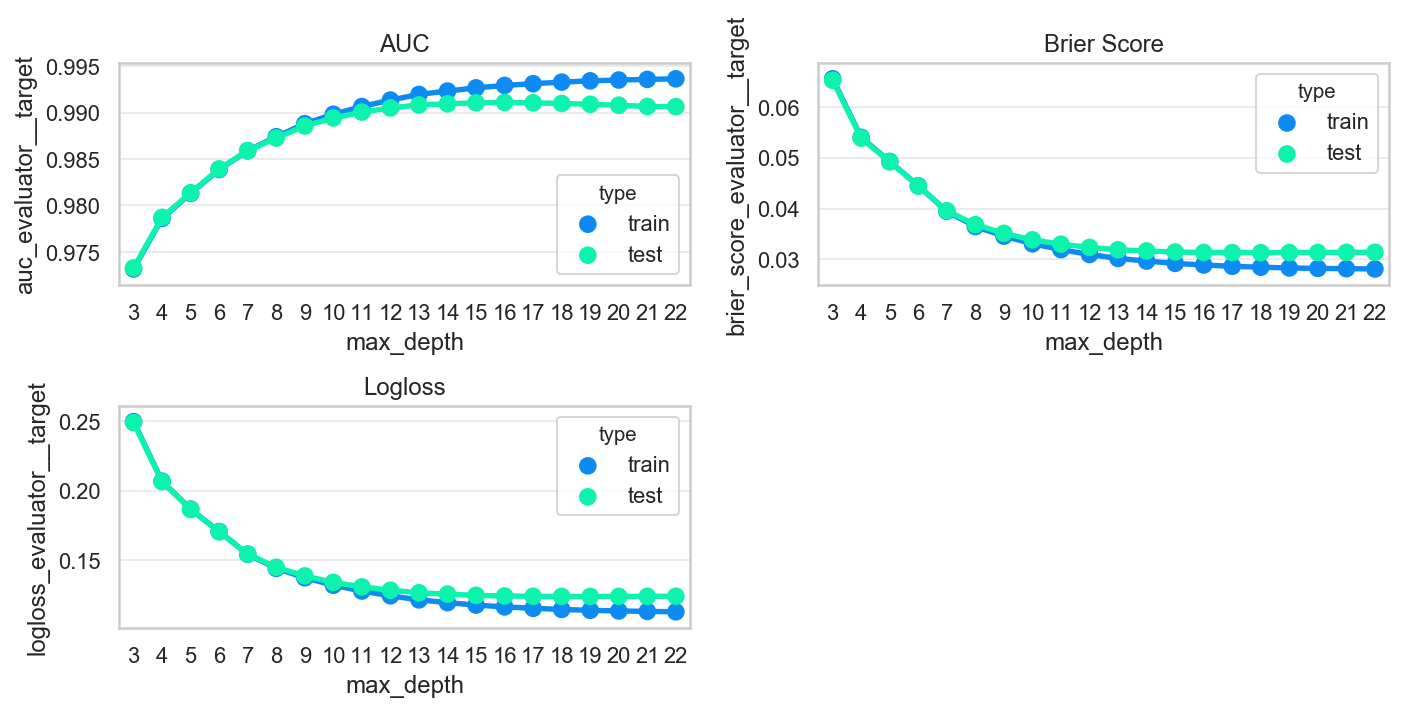
\includegraphics[width=1\textwidth]{res-ind2.png} 
    \caption{Individual impact of \textbf{\code{max\_depth}} on the \textit{BNG(kr-vs-kp)} dataset: one can observe that when $max\_depth > 14$ the model starts to overfit.}
    \label{fig:res-ind2}
\end{figure}

\begin{figure}[!h]
    \centering
    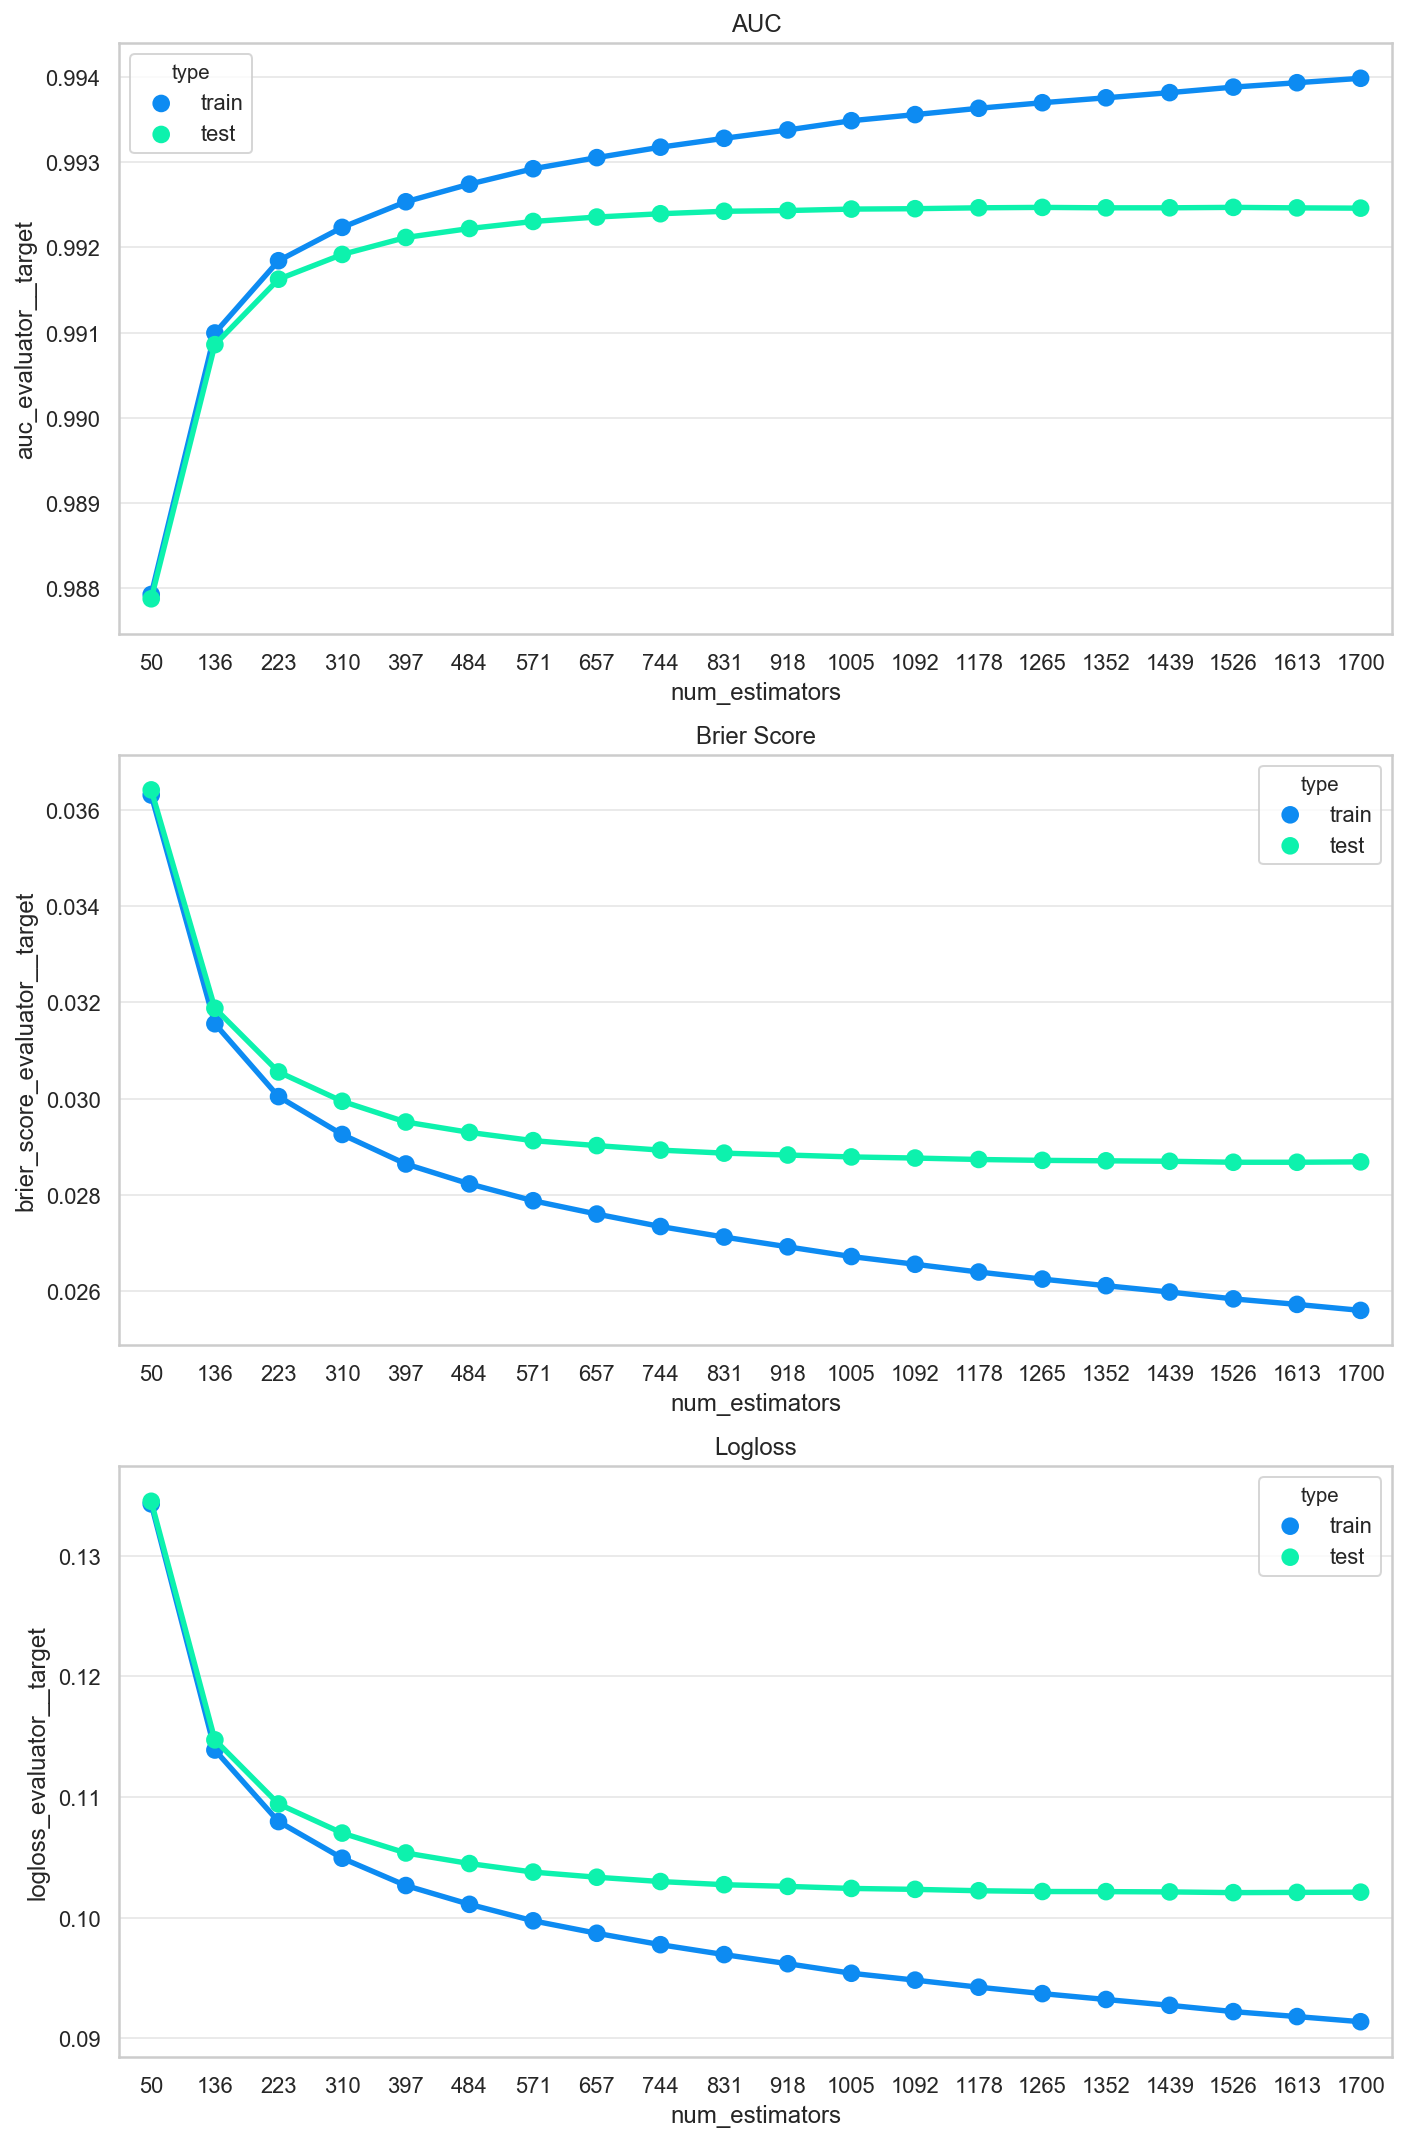
\includegraphics[width=1\textwidth, height=1.2\textwidth]{res-ind1.png} 
    \caption{Individual impact of \textbf{\code{num\_estimators}} on the \textit{BNG(kr-vs-kp)} dataset}
    \label{fig:res-ind1}
\end{figure}

\subsection{Hyperparameter Pairs Impact}

The second node of the hyperparameter tree defines all pairs of possible combinations of hyperparameters. In this study, these combinations are $MD_i \times LR_i$, $MD_i \times NE_i$ and $LR_i \times NE_i$. For example, in figure \ref{fig:res-mult1} one can see at the same time that a high \textbf{\code{num\_estimators}} combined with lower \textbf{\code{max\_depth}} have higher AUC on the test set (on this specific dataset), but at the same time low \textbf{\code{num\_estimators}} combined with high \textbf{\code{max\_depth}} also achieve high AUC. This is an interesting behavior that repeats in different hyperparameters combinations, and are easily detectable in the final general analysis looking at the treatment effect of each hyperparameter combination.

\begin{figure}[!h]
    \centering
    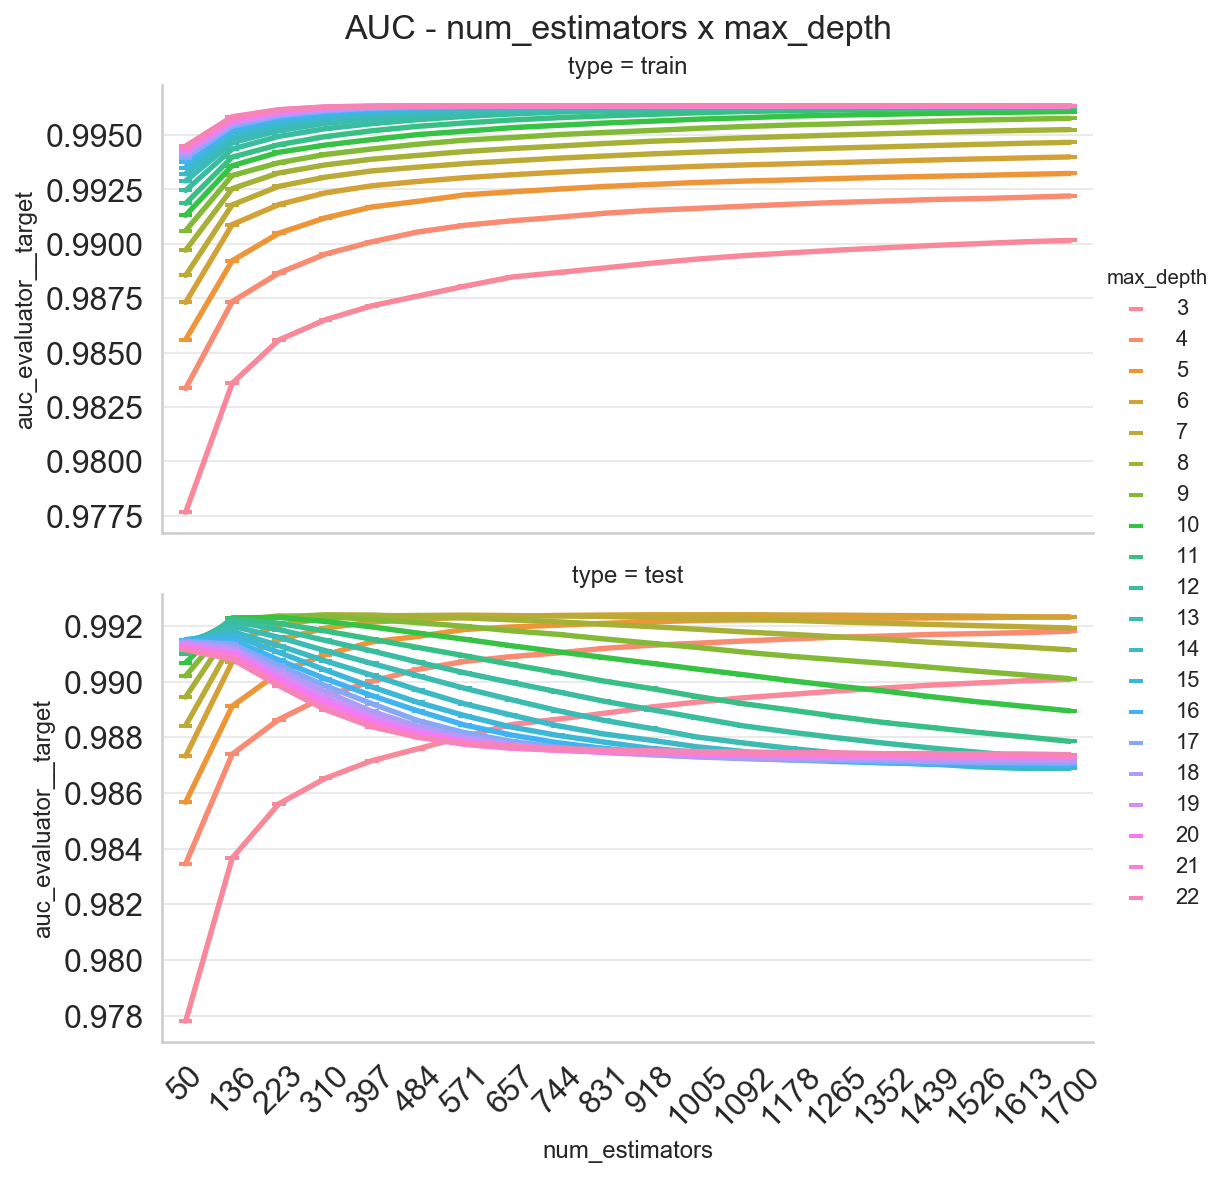
\includegraphics[width=1\textwidth]{res-mult1.png} 
    \caption{Pair impact of $MD_i \times NE_i$  on the \textit{BNG(kr-vs-kp)} dataset}
    \label{fig:res-mult1}
\end{figure}

On the other hand, when analyzing \ref{fig:res-mult2} the pair $MD_i \times LR_i$ doesn't show a clear inversion of the hyperparameters impact: one can only conclude that for \textit{BNG(kr-vs-kp)} lower \textbf{\code{max\_depth}} and high \textbf{\code{learning\_rate}} results in higher AUC (keeping the other hyperparameters the same). This is expected since the learning rate doesn't have the same ``overfit relationship'' as maximum depth and number of estimators have (explained in \ref{subsec:max-depth}).

\begin{figure}[!h]
    \centering
    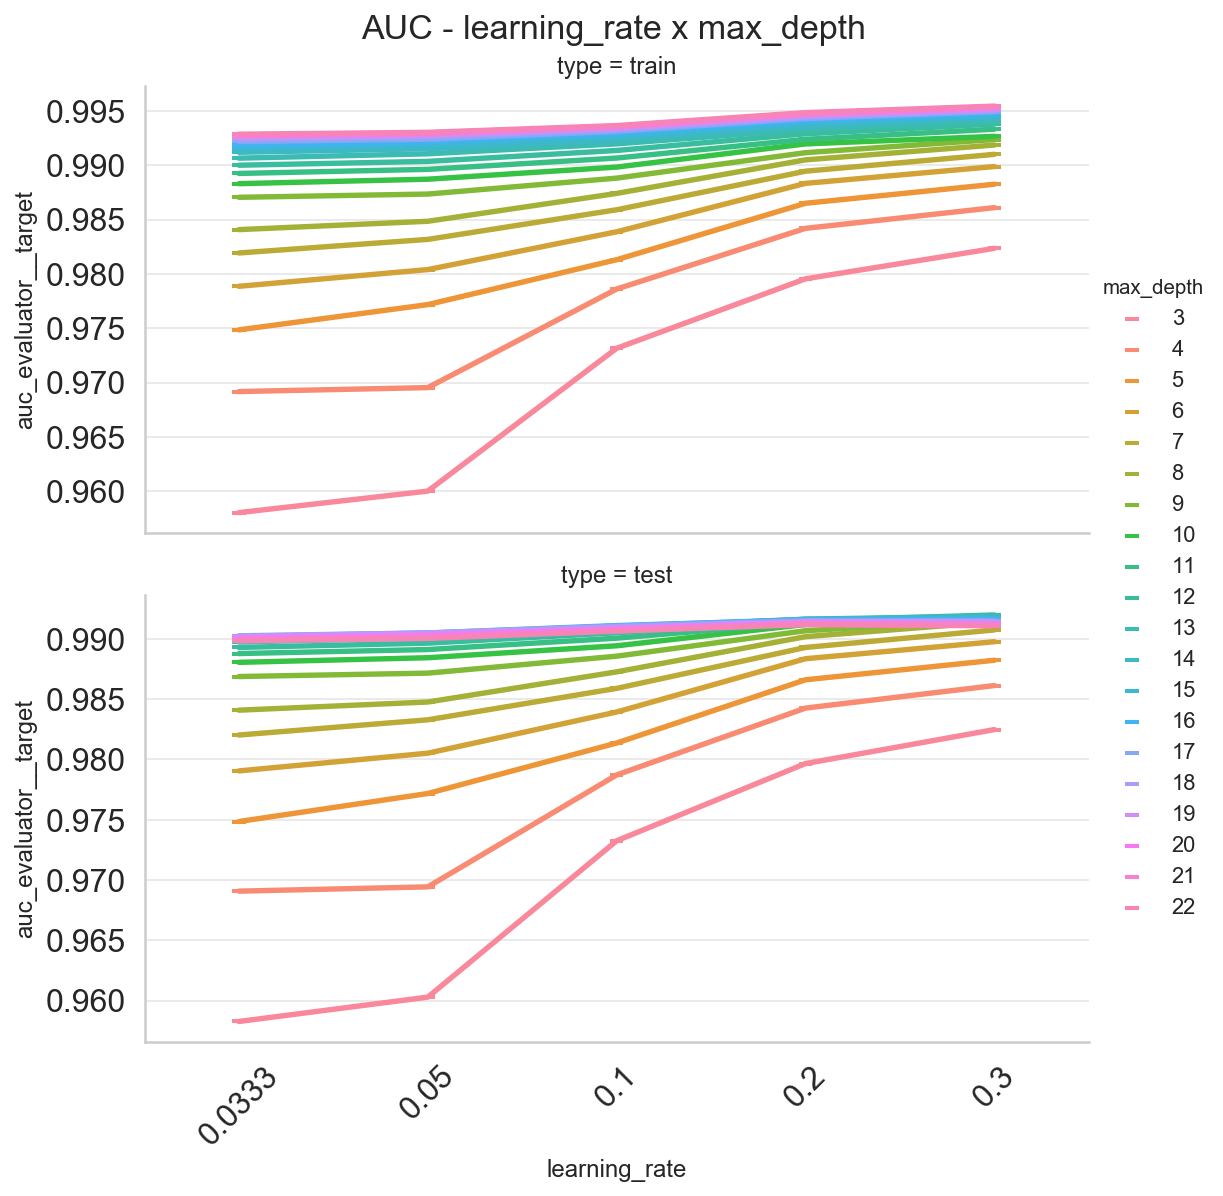
\includegraphics[width=1\textwidth]{res-mult2.png} 
    \caption{Pair impact of $MD_i \times LR_i$  on the \textit{BNG(kr-vs-kp)} dataset}
    \label{fig:res-mult2}
\end{figure}

\subsection{Hyperparameter Triples Impact}

Finally, each dataset is also run using all possible combinations of the studied hyperparameters, i.e. a classical Grid Search run using \code{num\_estimators}, \code{max\_depth} and \code{learning\_rate}. Results of AUC of the triple impact for  \textit{BNG(kr-vs-kp)} can be seen on figure \ref{fig:res-all1}.

\begin{figure}[!h]
    \centering
    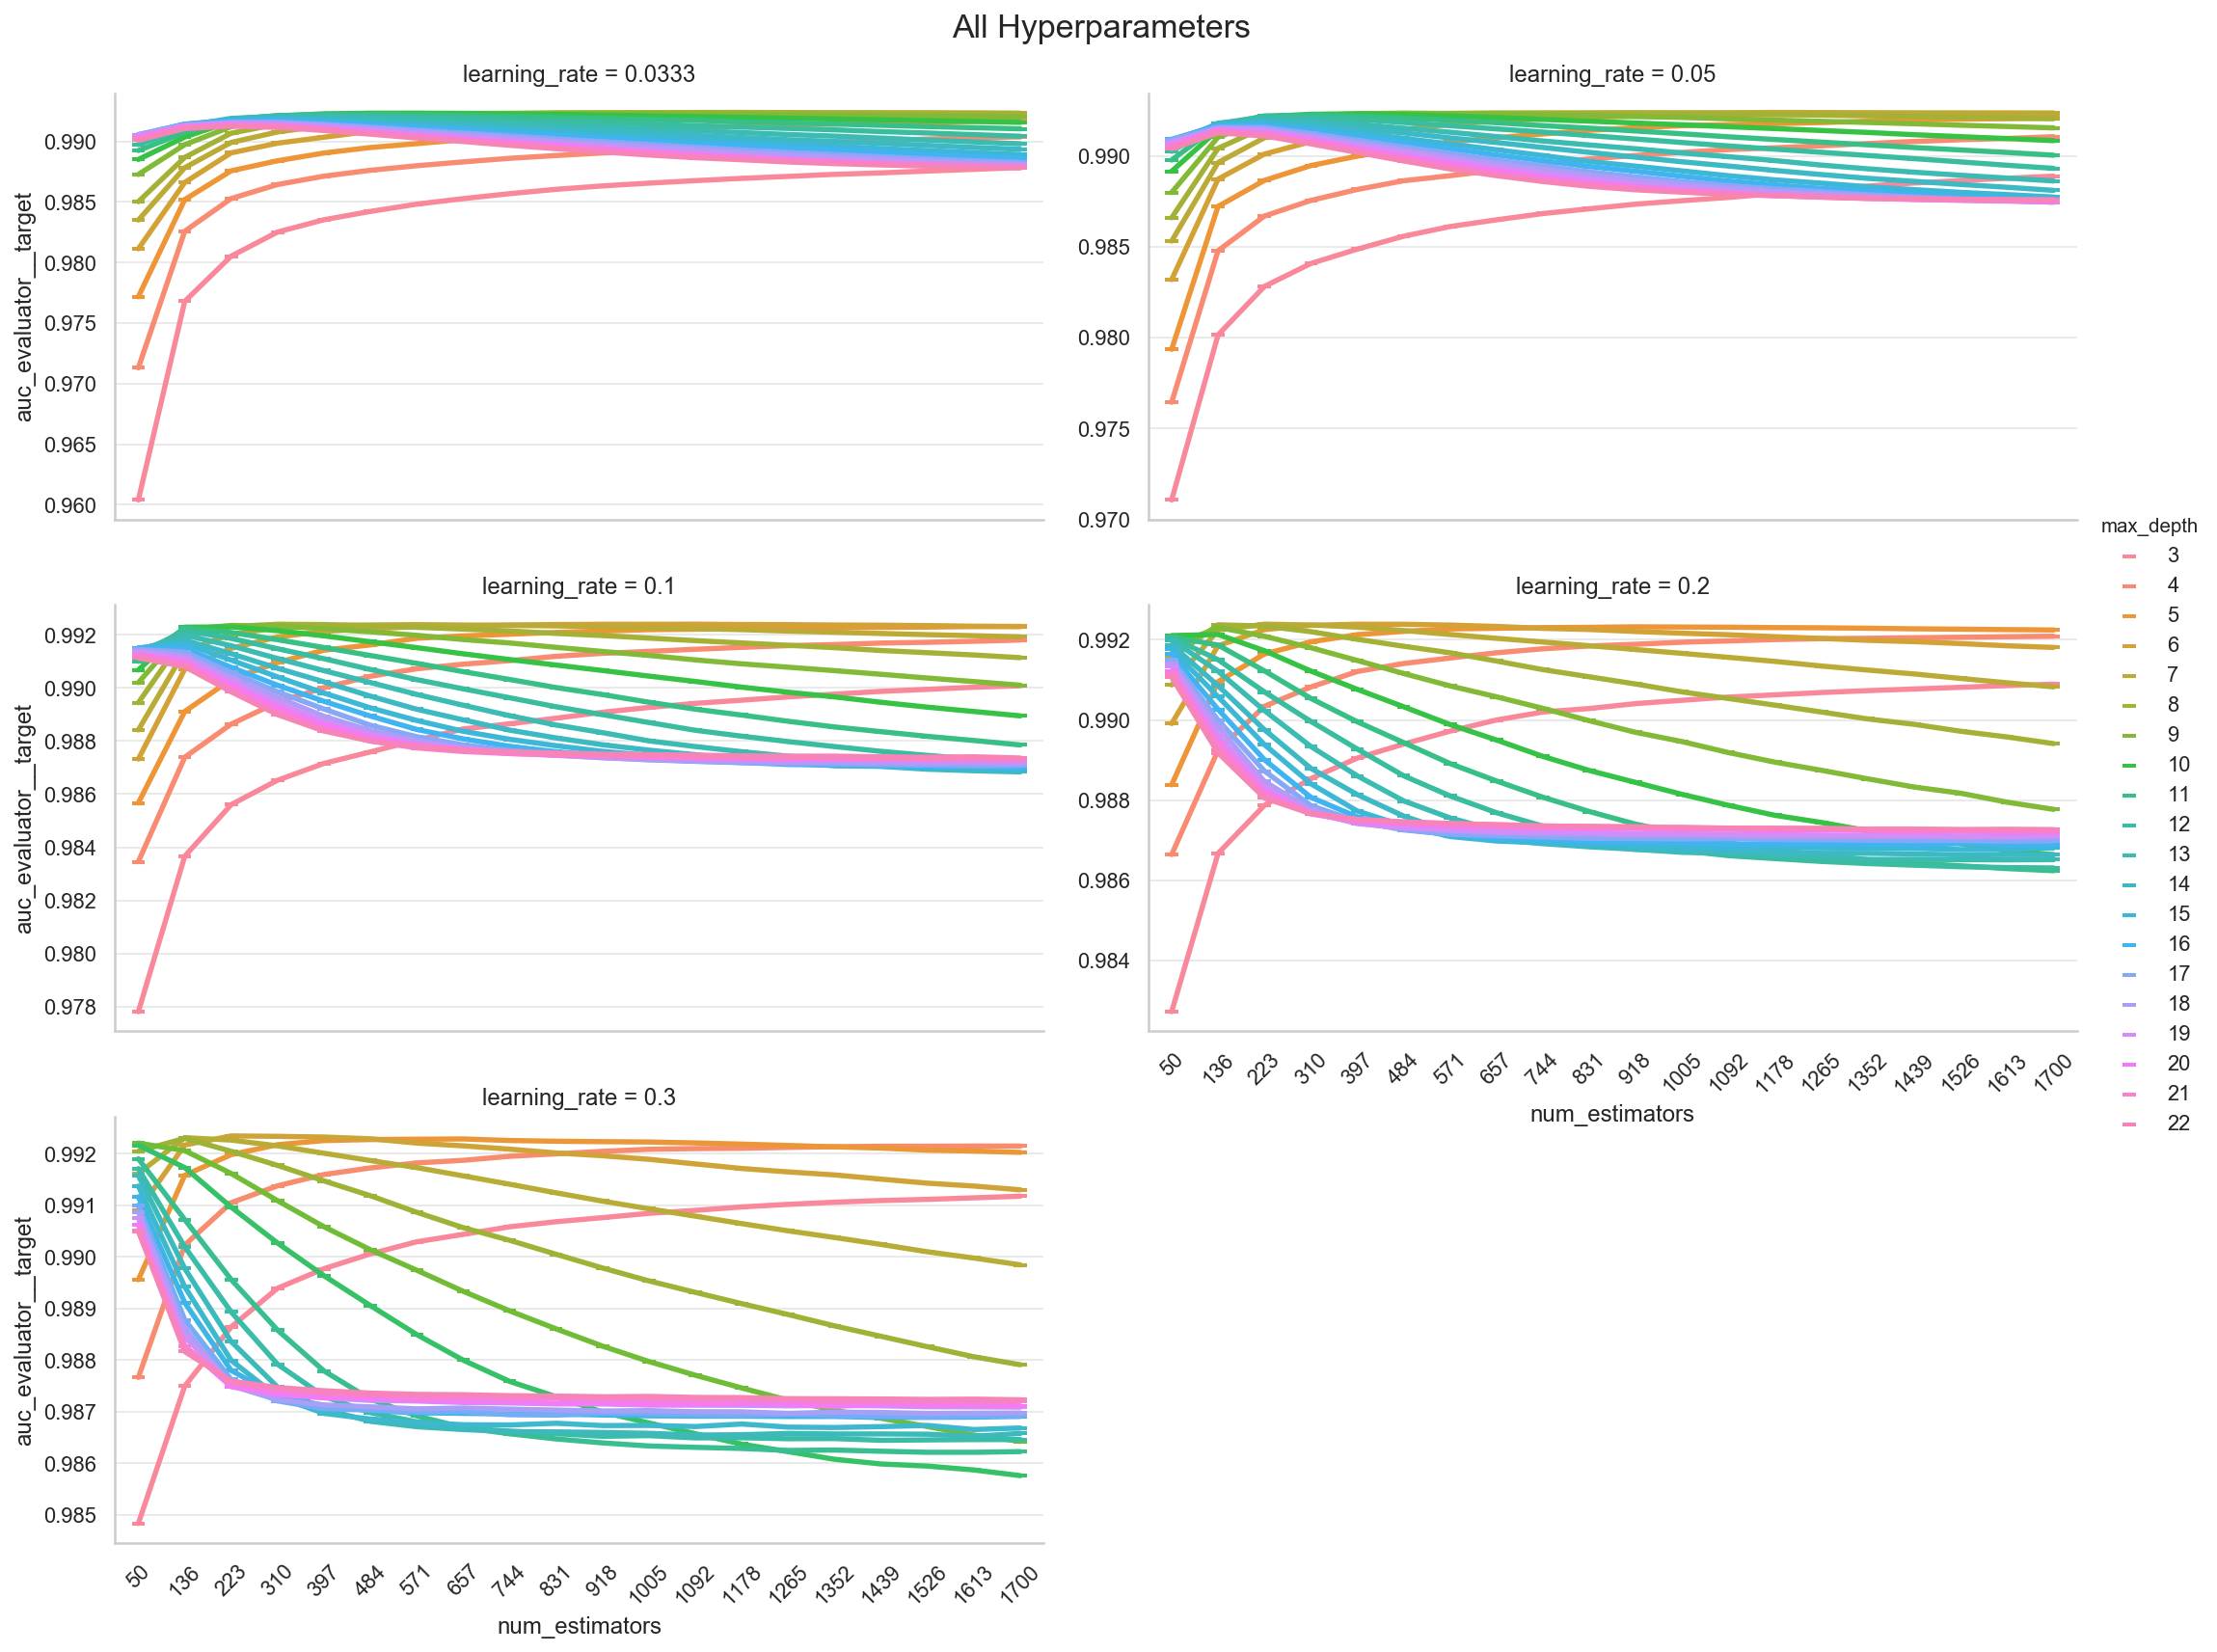
\includegraphics[width=1\textwidth]{res-everything1.png} 
    \caption{Triple impact of hyperparameters on the \textit{BNG(kr-vs-kp)} dataset, showing only \textbf{test} set AUC}
    \label{fig:res-all1}
\end{figure}

One of the inherent difficulties when analyzing these results is due to the high dimensionality of the results: Each experiment has at least the three hyperparameter values, plus three different metrics for each run. In section \ref{} this problem will be tackled, with an overview of the statistical techniques and analysis performed to compare and obtain insights into the impact on performance metrics.

%% ------------------------------------------------------------------------- %%
\section{Dataset aggregation and clustering}

To tie dataset characteristics to hyperparameters effect in the subsequent analysis, a variety of different measures were calculated in the dataset analysis process, explained in details in section \ref{dataset-aggregated-statistics} of chapter \ref{cap:study-methodology}. When analyzing all datasets's features characteristics, useful insights into the data can be found on it. First, a clear conclusion is that proportion of categorical features in the dataset is much higher than  other types (numeric, boolean or constants), as shown in figure \ref{fig:dset-pre1}, and that the most common cardinality is two categories for the categorical features\footnote{These categorical features could be encoded as the \textit{boolean} feature type, or vice-versa. In the study it was decided that boolean features are columns which had explicitly True and False as values.}, while few features have high cardinality (figure \ref{fig:dset-pre2}).

\begin{figure}[!h]
    \centering
    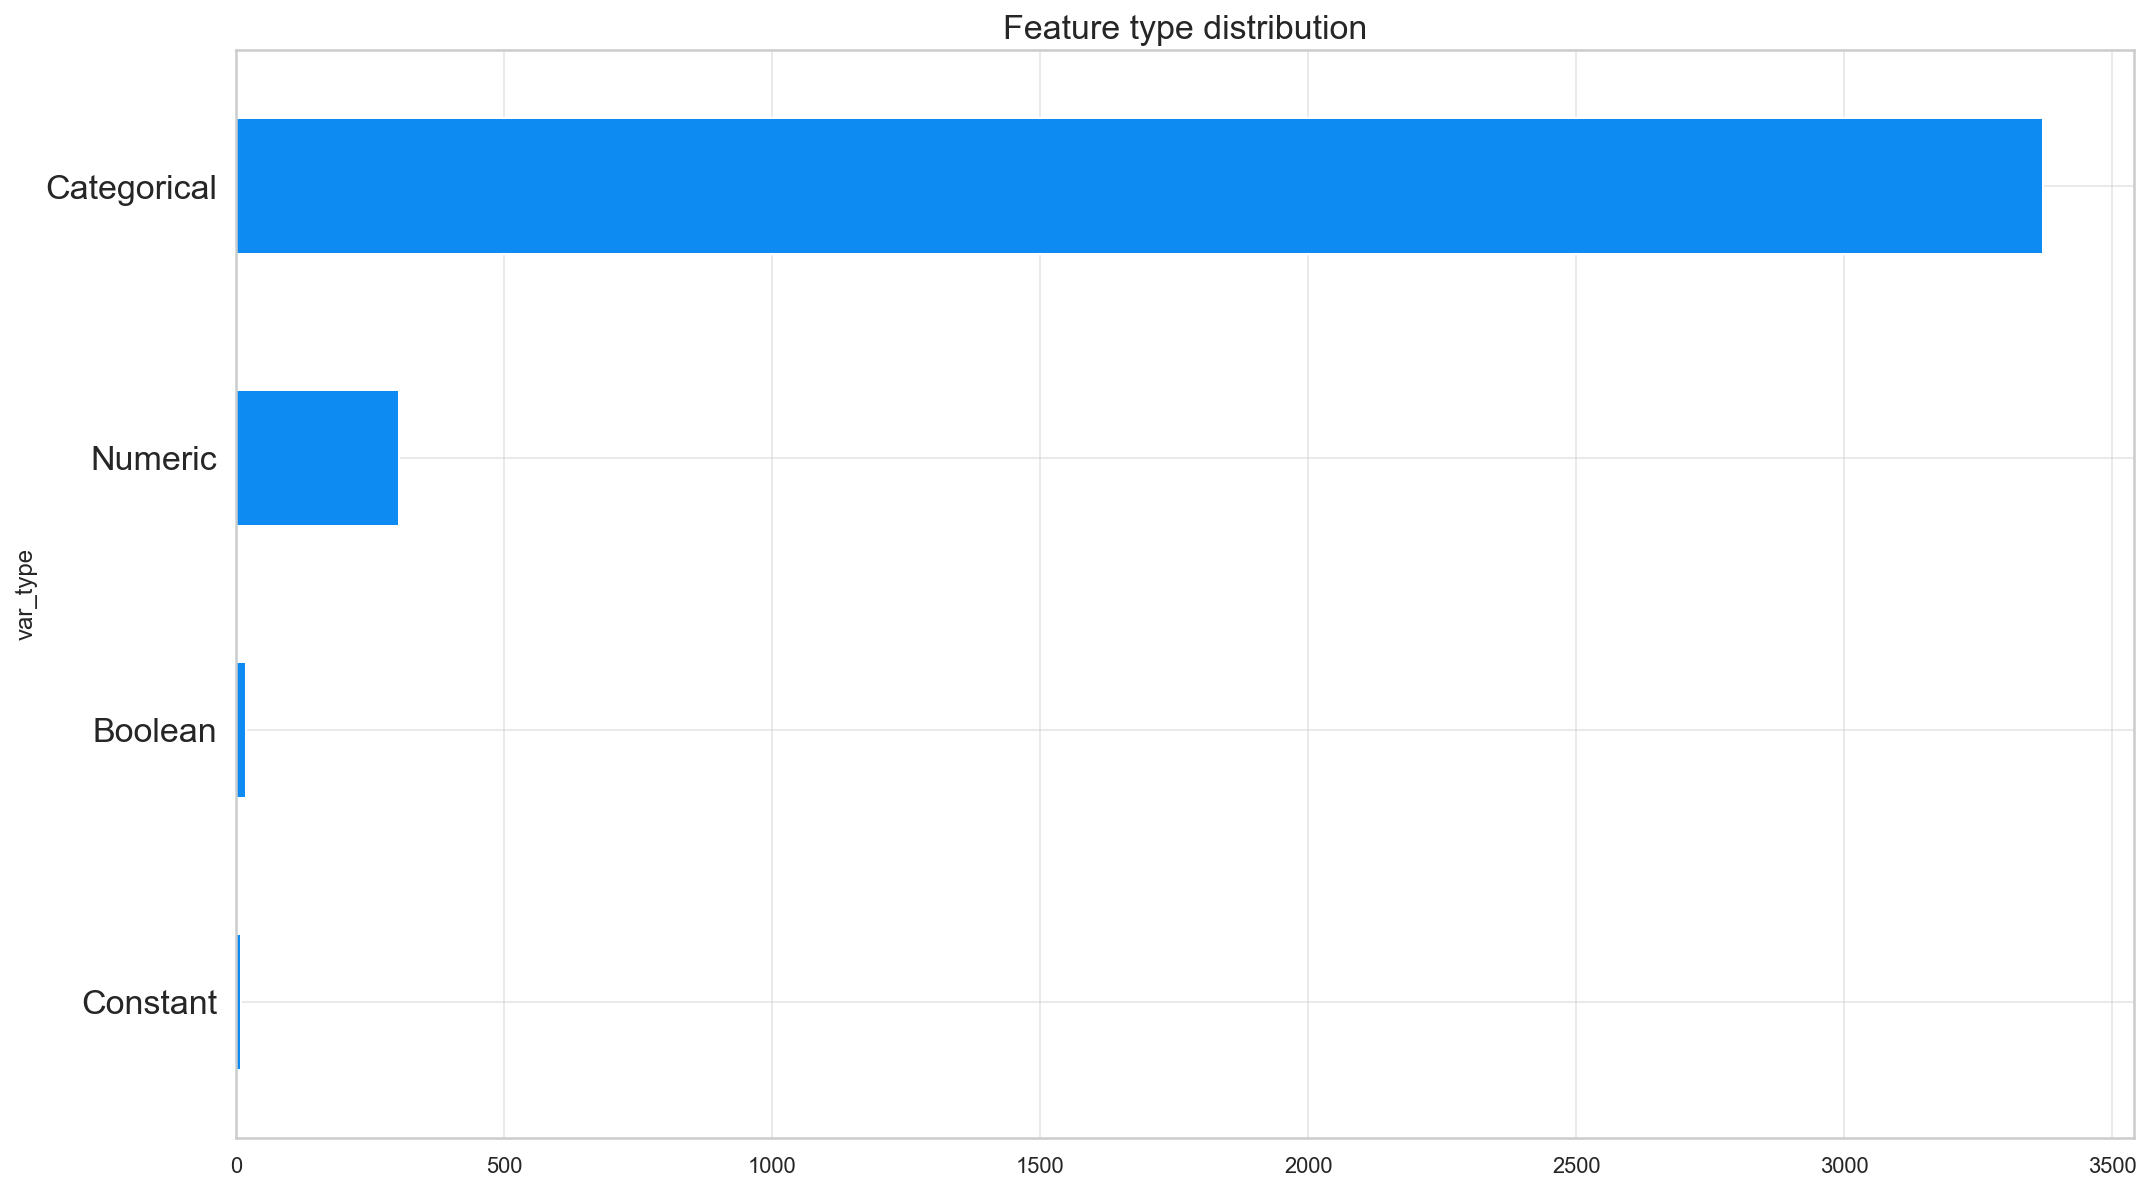
\includegraphics[width=.7\textwidth]{dset-pre1.png} 
    \caption{Feature types of the benchmark datasets}
    \label{fig:dset-pre1}
\end{figure}

\begin{figure}[!h]
    \centering
    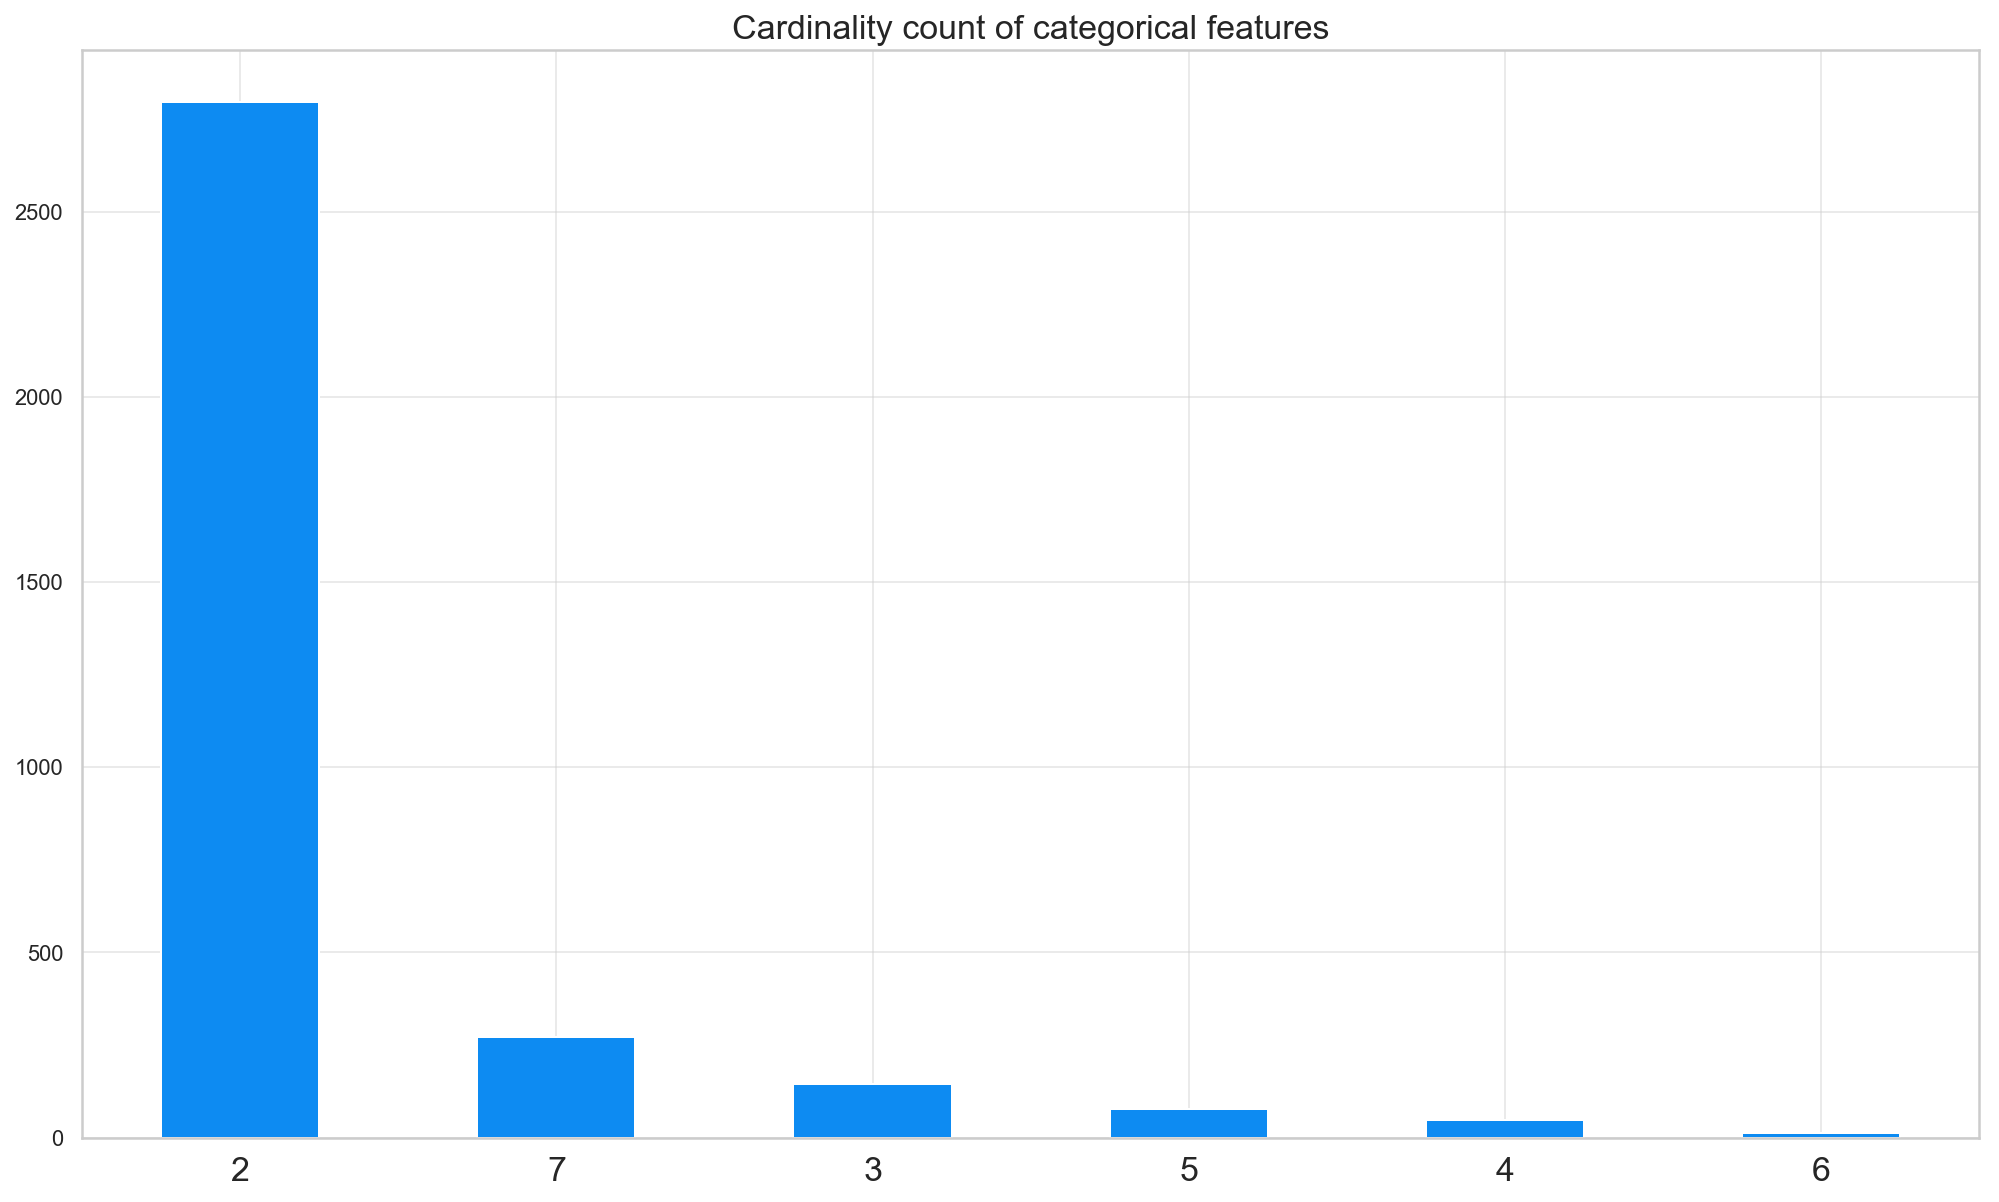
\includegraphics[width=.7\textwidth]{dset-pre2.png} 
    \caption{Cardinality of categorical features of the benchmark datasets}
    \label{fig:dset-pre2}
\end{figure}

Since the granularity of the statistics are feature-wise, all datasets were subjected to an aggregation process which combines the feature-wise statistics into \textit{dataset aggregated statistics}.
